\section{Thin strip graphs}

\subsection{$c$-strip graphs}

\begin{frame}{$c$-strip graphs}
\begin{definition}[$c$-strip graph]
  A $c$-strip graph (SG($c$)) is a unit disk graph such that the centers of the disks belong
  to $\{(x,y) : -\infty < x < \infty, 0 \leq y \leq c\}$.
\end{definition}
\pause

\begin{remark}
  SG($0$) = unit interval graph\\
  SG($\infty$) = unit disk graph
\end{remark}
\end{frame}

\subsection{Thin strip graphs}
\begin{frame}{Thin strip graphs}
  \begin{definition}[Thin strip graph]
    Thin strip graphs are defined as TSG $= \bigcap_{c > 0}$ SG($c$).
  \end{definition}
\pause

\begin{figure}
\centering
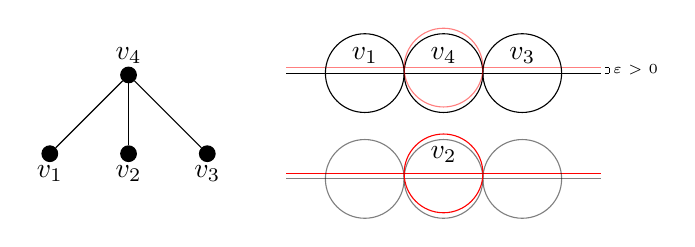
\begin{tikzpicture}
  \draw (-2,-0.7265) -- (2,-0.7265);
  \draw[red ,opacity = 0.5] (-2,-0.6565) -- (2,-0.6565);
  \draw  (-1,-0.7265) circle [radius=0.5];
  \draw[color=black] (-1,-0.5) node {$v_1$};
  \draw  (0,-0.7265) circle [radius=0.5];
  \draw[color=black] (0,-0.5) node {$v_4$};
  \draw  (1,-0.7265) circle [radius=0.5];
  \draw[color=black] (1,-0.5) node {$v_3$};

  \draw[red, opacity = 0.5] (0,-0.6565) circle [radius=0.5];
  \draw[color=black] (2.4386,-0.6898) node {\tiny $\varepsilon > 0$};

  % lines to describe distance (epsilon)
  \draw[very thin] (2.1,-0.6565) -- (2.1,-0.7265);
  \draw[very thin] (2.05,-0.6565) -- (2.1,-0.6565);
  \draw[very thin] (2.05,-0.7265) -- (2.1,-0.7265);

  \draw[opacity = 0.5] (-2,-2.07) -- (2,-2.07);
  \draw[red] (-2,-2) -- (2,-2);
  \draw[opacity = 0.5]  (0,-2.07) circle [radius=0.5];
  \draw[opacity = 0.5]  (1,-2.07) circle [radius=0.5];
  \draw[opacity = 0.5]  (-1,-2.07) circle [radius=0.5];
  \draw[red] (0,-2) circle [radius=0.5];
  \draw[color=black] (0,-1.765) node {$v_2$};

  \node[draw,circle,inner sep=2pt,fill,label distance=1cm] (v1) at (-4,-0.75) {};
  \draw[color=black] (-4,-0.5) node {$v_4$};
  \node[draw,circle,inner sep=2pt,fill,label distance=1cm] (v3) at (-4,-1.75) {};
  \draw[color=black] (-4,-2) node {$v_2$};
  \node[draw,circle,inner sep=2pt,fill,label distance=1cm] (v2) at (-5,-1.75) {};
  \draw[color=black] (-3,-2) node {$v_3$};
  \node[draw,circle,inner sep=2pt,fill,label distance=1cm] (v4) at (-3,-1.75) {};
  \draw[color=black] (-5,-2) node {$v_1$};
  \draw  (v1) edge (v2);
  \draw  (v1) edge (v3);
  \draw  (v1) edge (v4);

\end{tikzpicture}
\caption{Proof that TSG $\neq$ UIG.}
\label{fig:tsg_k13}
\end{figure}
\end{frame}

\subsection{Properties}

  \begin{frame}{Properties of thin strip graphs}
    \begin{theorem}
      MUIG $\subsetneq$ TSG $\subsetneq$ UUIG.
    \end{theorem}
    \begin{theorem}
      There is no constant $t$ such that SG($t$) $=$ TSG.
    \end{theorem}
    \pause
    \begin{remark}
      To prove these theorems, some forbidden induced subgraphs have been found.
    \end{remark}
  \end{frame}


\subsection{Open questions}

\begin{frame}{Open questions}
  \begin{block}{Forbidden induced subgraphs of TSGs}
    In order to study this graph, a characterization in terms of
    forbidden induced subgraphs has to be given. An exhaustive family of forbidden
    subgraphs could be researched.
  \end{block}
  \pause
  \begin{block}{Complexity of TSG recognition}
    Is the recognition of thin strip graphs $\mathcal{NP}$?
  \end{block}
  \pause
  \begin{block}{Complexity of other graph-theoretic problems}
    What can we say about the complexity of other graph-theoretic problems applied to
    thin strip graphs?
  \end{block}
\end{frame}
